\chapter{Sistema Web}

Os objetos de estudo aqui investigados apresentam em seus resultados poucas conclusões, seja no campo da espectroscopia, quanto na fotometria, seja quanto ao numero de objetos levantados nos bancos de dados, ou nenhum esclarecimento considerável relacionado aos parâmetros físicos associados aos jatos desta natureza. Dessa maneira, torna-se necessário a busca de novos objetos, novos estudos relacionados para o trabalho contínuo da pesquisa. Diante deste contexto, um sistema foi desenvolvido a fim de reunir os dados dos objetos bem como contemplar aqueles que carecem de informações. Deste modo, o cadastro de novos objetos da categoria estudada, poderá ser, em um só sistema, catalogados. Outro importante objetivo é fornecer a comunidade cientifica de forma concentrada as informações necessárias para a compreensão das Galaxias Peculiares com Jatos no visível. Para contemplar este objetivo, um sistema Web será adotado. 

Nesse capítulo apresentamos as principais ferramentas envolvidas que colaboraram com o desenvolvimento do sistema. É certo que, no campo relacionado ao desenvolvimento de sistemas, a gama de ferramentas e linguagens se estende. A escolha das linguagens aqui apresentadas, justifica, para um primeiro instante,  sua consolidação e robustez. Uma dessas linguagens aqui empregadas é o PHP que em servidores Web é a linguagem que ainda domina \cite{hills2013empirical}.

Logo, para o desenvolvimento do sistema utilizaremos as tecnologias Web, HTML, CSS, PHP e Javascript. A linguagem que assegura a criação de paginas Web é a linguagem de marcação HTML (do inglês Hypertext Markup Language). É através dela que as páginas são estruturadas e o conteúdos organizados. Isso é possível mediante o uso de 'tags'. Com isso, parágrafos, tabelas e títulos são criados e posicionados. São por meio das 'tags' que o corpo da página é formatado. Um banco de dados também foi modelado e construído utilizando o Sistema Gerenciador de Banco de Dados Mysql e o servidor web Apache.

Para o site, um layout foi construído, levando em consideração os requisitos planejados para o sistema, a qual falaremos na seção \ref{sec:requisitos}. Originalmente o conteúdo do website foi escrito na língua inglesa, de modo que o mesmo tenha uma maior inserção no campo acadêmico. Deste modo o website provém de seções em um menu que dispõe ao usuário módulos do sistema onde encontram-se formulários de consulta para os objetos de interesse.
Para os objetos que ora dispomos, um total de 125 espectros já foram inseridos no banco de dados de forma automática. Para tal, uma pré-modelagem foi montada e um ambiente no site criado para inserí-los.
Como o objetivo do sistema é, justamente fornecer a comunidade pesquisas relacionadas aos objetos, tratamos de oferecer em primeira mão, as informações fotométricas que anteriormente foram produzidas segundo os Capítulos \ref{subsec:image_mult}, \ref{subsec:spec_mult} e os espectros tratados e corrigidos por redshift. Todos os arquivos foram carregados no Banco de dados via PHP para o gerenciador Mysql. Uma vez carregados, o sistema dispõe todos os arquivos via pesquisa montados em formulários Web.

Mediante este objetivo descrito acima, foi percebido a necessidade de, também, modelar o sistema e  disponibilizar todos os dados de forma dinâmica. Para todos os objetos, 'Bokeh', uma biblioteca da linguagem Python, gera plots para cada espectro. Deste modo, além das informações, referências, posições disponíveis ofertadas pelo sistema, o mesmo contempla também plotagens dos espectros disponíveis no banco de dados. Cada plotagem é gerada de forma dinâmica, na própria pagina de conteúdo, não se fazendo necessário gerar para cada objeto um plot salvo em banco. Uma característica didática, presente no sistema de plotagem 'Bokeh', se refere a função que permite ao usuário interagir com o gráfico, podendo dessa forma, investigar no próprio site, posições ou áreas especificas do espectro via Web. A imagem abaixo ilustra um exemplo:

\begin{figure}[H]
	\centering	
    \caption{Plot no Sistema}
    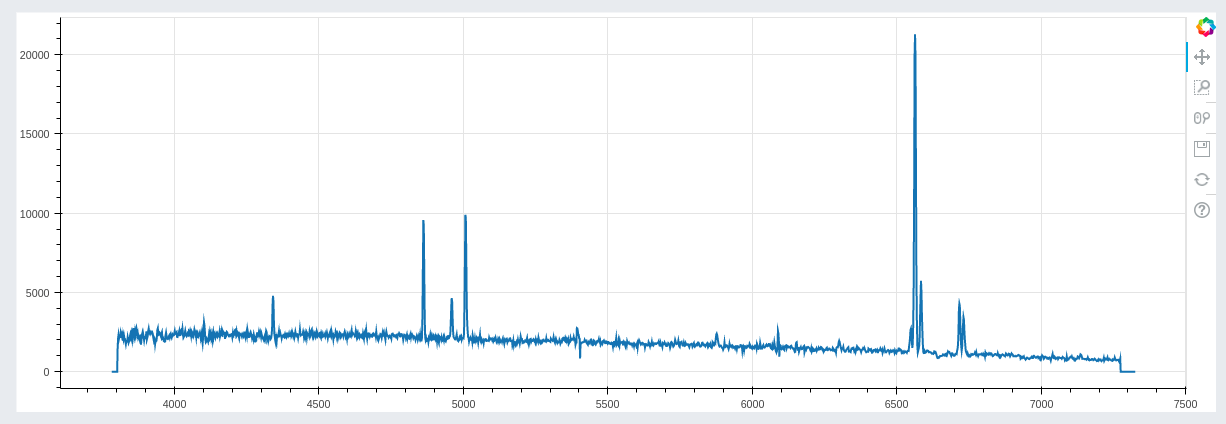
\includegraphics[width=1.0\textwidth]{figuras/spec_plot.png}
   	\begin{center}
        \normalsize Fonte: Próprio Autor \\Plotagem de um espectro gerado pelo Bokeh, uma biblioteca de gráficos feita em Python
    \end{center}
	\label{fig:sbmt-moses}
\end{figure}

Para a busca dos objetos, seja relacionado as informações fotométricas ou espectroscópicas, duas seções foram criadas para tal pesquisa. Dois modos foram disponibilizados para a pesquisa, sendo a primeira pelo nome do objeto, devendo ser o nome originalmente catalogado por Arp \& Madore. O segundo modo pode ser feito via pesquisa de posições em coordenadas equatoriais (ascensão reta e declinação). A pesquisa retorna uma imagem semelhante a figura \ref{fig:fotometry_mosaic} ou \ref{fig:1146-270} respectivamente. Além deste, também uma lista de parâmetros e referencias ligada ao objeto será apresentada. Tais parâmetros foram cadastrados via formulário web. O resultado apresenta os seguintes parâmetros:

\begin{itemize}

\item Referencias - Artigos e produções bibliográficas de estudo do objeto, no formato bibtex, e um link para cada fonte publicada;

\item Redshift - Valor referente ao desvio para o vermelho;

\item Magnitude – Medida do brilho dos objetos na qual um aumento de uma magnitude indica uma dimuição no brilho por um fator 2,512, nas diversas bandas fotométricas;

\item Classificação – Referente ao tipo morfológico do objeto.
\end{itemize}

Referente as pesquisas relacionadas à espectroscopia, uma seção também foi criada chamada “Database” onde, da mesma forma que fizemos para a pesquisa fotométrica, podemos também empregar esta pagina. Neste caso, a saída será um objeto para download no formato FITS, as posições e um botão para o plot do espectro. 


\section{Cadastro de Usuários}

Para o gerenciamento do sistema, empregamos um modo de cadastro de usuários que, desta forma, poderão se cadastrar e editar o conteúdo. Para o cadastro, um script em PHP foi escrito para validar e receber os valores passados. Para as validações, é exigido para o cadastro, um email e senha com um numero mínimo de caracteres. Para o email, este será apenas válido se contiver caracteres obrigatórios como “@” e o ponto. Já para cadastrar novos usuários, um sistema de token foi desenvolvido, visando o controle de participantes no sistema. Para tal, uma função feita também em PHP foi escrita para gerar números e letras de forma aleatória. Uma vez feito isso, o administrador poderá compartilhar com o usuário de interesse e efetuar o cadastro. Isso evita usuários indesejados e de forma segura manter a integridade do sistema. Dessa forma o administrador manterá o controle e demais pessoas contribuirão com o trabalho, em publicações e atualizações.

Uma vez que um usuário é cadastrado, uma tupla\footnote{Basicamente, o que diferencia a 'Estrutura de Dados Lista' da 'Estrutura de Dados Tupla', é que a primeira pode ter elementos adicionados a qualquer momento, enquanto que a segunda estrutura, após definida, não permite a adição ou remoção de elementos.} (ou seja, uma lista imutável) é gerada no banco de dados. No que segue, apresentamos um exemplo da função em PHP que,  quando conectado ao banco de dados, enviará comandos SQL para a execução de um novo usuário no sistema:


\begin{comment}
\begin{lstlisting}[caption={Codigo PHP para inserção de usuários}]
<?php
// Incluir o arquivo de conexao com o mysql e o banco de dados
include 'conexao.php';

// inserindo varios registros
mysqli_query($conn, "INSERT INTO user (codigo, nome) VALUES (1, 'Joao')");
mysqli_query($conn, "INSERT INTO user (codigo, nome) VALUES (2, 'Carla')");
mysqli_query($conn, "INSERT INTO user (codigo, nome) VALUES (3, 'Anna')");
mysqli_query($conn, "INSERT INTO user (codigo, nome) VALUES (4, 'Matheus')");
mysqli_query($conn, "INSERT INTO user (codigo, nome) VALUES (5, 'Laura')");

//encerra conexao com o banco de dados
mysqli_close($conn);
?>
\end{lstlisting}
\end{comment}

\section{Análise de requisitos}
\label{sec:requisitos}
 
Os requisitos do sistema se referem as funções, atividades e processos que contemplam as necessidades do projeto para o sistema durante seu desenvolvimento até sua conclusão. Em geral, os requisitos são classificados em dois modos: o primeiro de cunho funcional, isto é, que define exatamente o que o sistema deverá fazer e como deve se comportar diante da necessidade do usuário, enquanto o segundo deverá levar em consideração propriedades referentes à segurança, portabilidade, desempenho e usabilidade. Abaixo estão listados os requisitos citados:

Requisitos Funcionais:

\begin{itemize}
\item RF1: O sistema permite o acesso ao download dos arquivos sem comprometer a segurança do sistema;
\item RF2: O sistema deve ser capaz de aprovar novos usuários via tokem;
\item RF3: O sistema deve ser capaz de enviar dados ao BD;
\item RF4: O sistema deve ser capaz de exibir os dados requeridos pelo usuário como as imagens, espectros, plots dos espectros e fontes de cada dado;
\item RF5: O sistema deve ser capaz de efetuar login e cadastrar novos dados;
\item RF6: O sistema deve ser capaz de gerar arquivos bibcode.txt referente a cada objeto contendo suas devidas referencias.
\item RF7: A inteface gráfica Web deverá ser responsiva, permitindo ajuste do layout automático para diferentes tamanhos de tela.
\end{itemize}

Requisitos Não Funcionais:

\begin{itemize}
\item RNF01: O sistema deve ser de fácil entendimento e usabilidade para professores e alunos;
\item RNF02: O sistema deve ser capaz de funcionar em qualquer ambiente, como celulares e tablets;
\item RNF03: A aplicação deverá estar disponível na língua inglesa;
\item RNF04: O sistema poderá ser atualizado sempre que necessário;
\end{itemize}

\section{Modelagem do Sistema}

Para elaborar a documentação, construir suas etapas visualizar os procedimentos necessários de forma lógica, submetemos o processo de sua construção os procedimentos da modelagem UML, que é a linguagem padrão para a elaboração de projetos. Dessa forma é possível padronizar os passos e estruturas que um sistema requisita. 

\subsection{Diagrama de Caso de Uso}

Diagrama de caso de uso representa em alto nível como o sistema deverá se comportar em relação a um determinado individuo, chamado usualmente de 'Ator'. De forma direta, documenta o que o sistema faz em relação ao usuário e suas interações. Ele busca apresentar na perspectiva do usuário, as funcionalidades e recursos do sistema. O diagrama (ver figura \ref{fig:uso}) foi montado no inicio da modelagem do sistema, juntamente com a analise de requisitos.

\begin{figure}[H]
	\centering	
    \caption{Diagrama de Caso de Uso}
    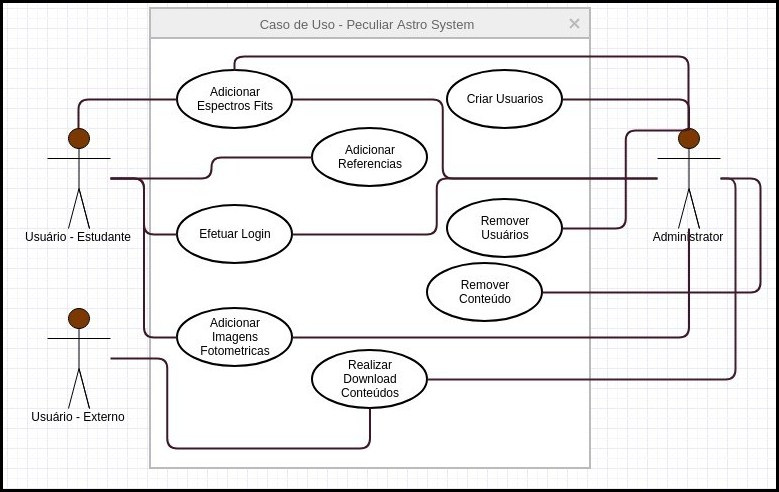
\includegraphics[width=1.0\textwidth]{figuras/caso_de_uso.png}
   	\begin{center}
        \normalsize Fonte: Próprio Autor \\Digrama representando relação de autores e funções do sistema
    \end{center}
	\label{fig:uso}
\end{figure}

\section{Modelagem do Banco de dados}

A modelagem do banco de dados foi baseado no modelo Entidade Relacionamento (MER). Dessa forma, podemos descrever os objetos (Entidades) envolvidos no projeto, bem como também suas características. A ideia do modelo, permite, de forma objetiva, estabelecer o relacionamento entre as entidades e as características que este apresenta. Neste modelo cada registro de tabela é distinto de todos os outros, e suas relações estabelecidas mediante um tipo de atributo, chamada 'chave primaria', que pode ou não relacionar as tabelas.  É mediante tal modelo que, de forma abstrata, qual forma e estrutura a aplicação do sistema terá. Tais relacionamentos foram representados mediante o 'Diagrama Entidade-Relacionamento'. 

\subsection{Diagrama de Entidade-Relacionamento}

O diagrama de entidades consiste de 7 tabelas e com o auxílio do software 'Mysql Workbench', o diagrama do banco de dados foi montado. Nesta ideia, o sistema poderá guardar os dados de forma estruturada e organizada e onde todas as tabelas estão relacionadas.
A seguir a figura ilustra o diagrama:

\begin{figure}[H]
	\centering	
    \caption{Diagrama Entidade-Relacionamento}
    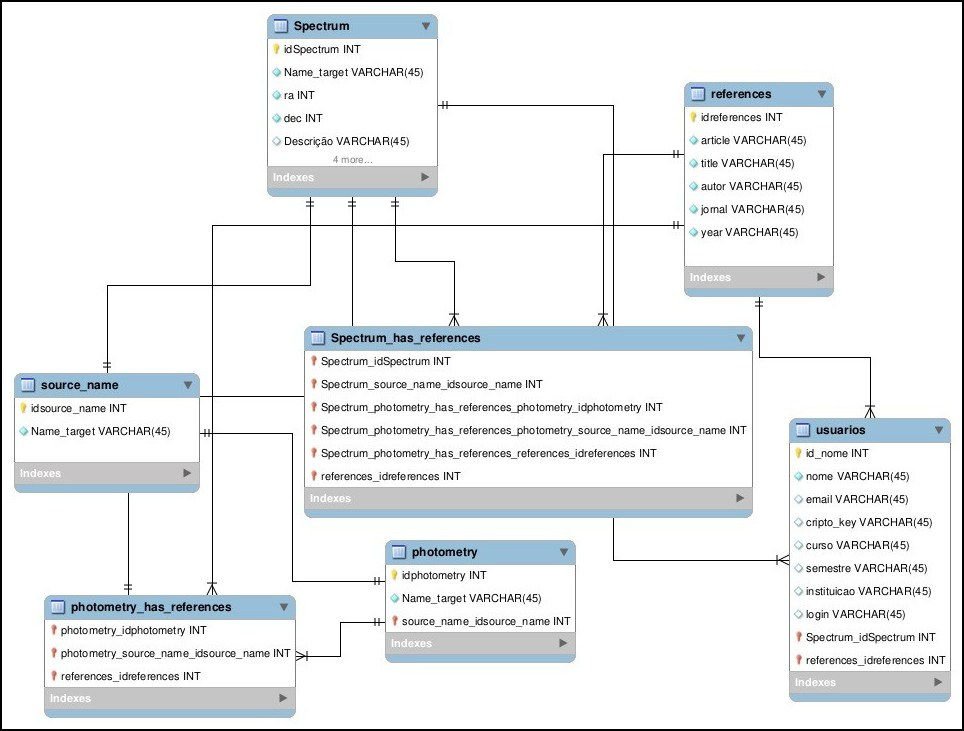
\includegraphics[width=0.8\textwidth]{figuras/modelo_er_latex.jpg}
   	\begin{center}
        \normalsize Fonte: Próprio Autor \\Digrama representando as principais tabelas e como estão conectadas.
    \end{center}
	\label{fig:sbmt-moses}
\end{figure}

\section{Desenvolvimento Front-end}

Quando falamos em Front-end, nos referimos ao desenvolvimento dos componentes subjacentes para o fornecimento da interface ao usuário. É através dele que trabalhamos o layout, design e apresentação de um sistema web ou aplicativo. No caso especifico desta pesquisa, usamos uma coleção de ferramentas, 'frameworks' e algumas linguagens de programação para trabalhar na estrutura lógica do comportamento das funções do sistema para o usuário. Uma das tecnologias Web envolvidas nesse projeto foi a linguagem Javascript. Com ela é possível trabalhar no nível "Client-side", ou seja, rodar processos que são executados no computador do cliente, mais especificamente no 'browser', executar estruturas de programas, fazendo da página um ambiente inteligente.
Para o menu principal, slides e roda-pé, o uso de um framework Web chamado 'Bootstrap', foi usado para gerar de forma intuitiva cada parte destas seções. Um framework é uma abstração que une códigos e projetos para promover uma funcionalidade. Neste caso, o Bootstrap une a linguagem de marcação HTML, linguagem de folhas de estilo CSS, e Javascript, tornando assim a página fluida, dinâmica e responsiva. Responsividade, como citado anteriormente, é uma técnica usada através da liguagem CSS para manter a ordem e organização de como as partes do site se moldam de acordo com uma plataforma. Com o advento das plataformas mobile, o uso de sites por meio de celulares e tablets forçou no desenvolvimento dessa tecnica através do recurso conhecido como 'media queries' do CSS. Neste caso o sistema desenvolvido neste projeto pode ser usado não só em computadores comuns, mas nas diversas plataformas encontradas. O Bootstrap unindo essas linguagens, nos permitiu desenvolver toda a parte gráfica do sistema de forma rápida e eficiente, poupando o desenvolvimento de massivas linhas de código. A imagem a seguir ilustra como essa parte do sistema se encontra até o momento.

\begin{figure}[H]
	\centering	
    \caption{Layout do Sistema}
    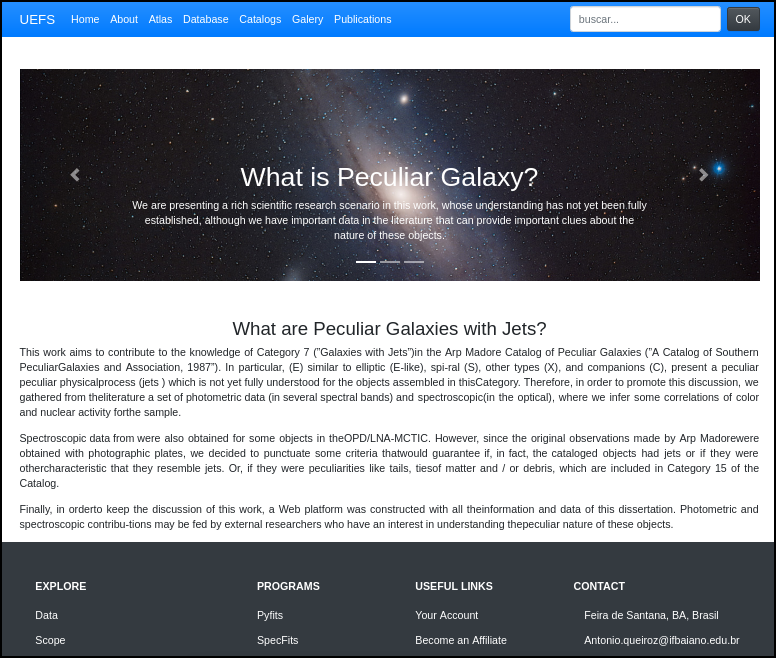
\includegraphics[width=1.0\textwidth]{figuras/site-latex-final.png}
   	\begin{center}
        \normalsize Fonte: Próprio Autor \\Pagina inicial do site
    \end{center}
	\label{fig:sbmt-moses}
\end{figure}

\section{Desenvolvimento Back-end}

De forma superficial, podemos já vislumbrar como o sistema se apresenta visualmente ao usuário. Porém, as estruturas e tarefas que não são controladas nem visíveis pelo usuário, é chamado de desenvolvimento Back-end. Esta parte é onde cuidaremos do banco de dados, como o sistema coleta os dados, e como são computados. 
Uma das linguagens usadas para a construção dessa aplicação foi o PHP (acrônimo recursivo do inglês: Hipertext Processor), uma linguagem open source, com a capacidade de inserção de seus códigos em paginas HTML. Através dela, conectamos ao Mysql, inserimos os dados ao banco ou consultamos valores. O Mysql é um SGBD (Sistema Gerenciador de Banco de Dados). O motivo de sua escolha se dá pela fácil implementação, fácil acesso, inteface simples e protegido sob licença de software livre , desenvolvida pela GNU. 
Para a implementação do sistema usamos o servidor HTTP Apache que é responsável por disponibilizar páginas e todos os recursos para os usuários. 

\section{Implantação do Sistema}

As tecnologias envolvidas na implementação do sistema, já são, de certo modo, consagradas por grande parte da comunidade tecnológica. Após o sistema criado e boa parte de seus módulos em funcionamento, restou então, colocá-lo em uma plataforma de hospedagem e disponibilizar seu conteúdo. Sendo assim, o serviço de hospedagem usado é o Webhost, que oferece suporte ao PHP, Mysql suas tecnologias e também sendo possível hospedar um sistema gratuitamente. Desta forma, pelo endereço \url{https://astrouefs.000webhostapp.com/} é possível acessar o site. O endereço e domínio agora citado está apresentado provisoriamente, e deverá ser mudado assim que um novo domínio for adquirido.

